\section{Getting Started}
\label{sec:getting-started}

\subsection{Setup}
\label{sec:setup}

The Scenario Checker is installed into Rodin from the plugin update site in the normal way.
It is located under the Utilities category.

The Scenario Checker depends on (and will install elements from)
\itemize{
\item ProB - de.prob
\item ProB Support - ac.soton.eventb.probsupport
\item Event-B EMF framework - org.eventb.emf
}

\emph{At the time of writing, the Scenario Checker is only available as a prototype on the soton prototypes update site.}

\subsection{Perspectives}
\label{sec:perspectives}

The Scenario Checker defines a perspective which includes the Scenario Checker Control and Scenario Checker State views as well as the ProB history view which is useful to see the executed scenario (including internal events). 
The ProB state view is also open (stacked behind Scenario Checker State) in case a more detailed view of state is needed.

The Scenario Checker views are also contributed to the BMotion Studio Run perspective and are available as short cuts on the Event-B perspective.

\subsection{Starting}
\label{sec:starting}

The Scenario Checker is started using the context menu of a machine as shown in Fig.~\ref{fig:starting}.
I.e. by right clicking on a machine in the Event-B navigator and selecting the \textbf{Scenario Checker} menu item.
An alternative is to ensure that at least one of the scenario views is opened (e.g. by selecting the Scenario Checker perspective) and then using the start toolbar button of the ProB support plug-in. 
(This is the green running man shown circled in red in \ref{fig:starting}).
In both cases, the ProB support plug-in will be used to launch the scenario checker as well as any other participating animation plugins that are opened representing the same machine.
For example, in Fig.~\ref{fig:starting}, the BMotion Studio visualisation and state-machine will also start animating if they are linked to the machine that is being started for the Scenario Checker.

The Scenario Checker should be stopped by selecting the machine again and using the red standing man toolbar button.
If another machine is started via the ProB support plugin, any current animation will first be stopped.


\begin{figure}[!htbp]
  \centering
  \ifplastex
  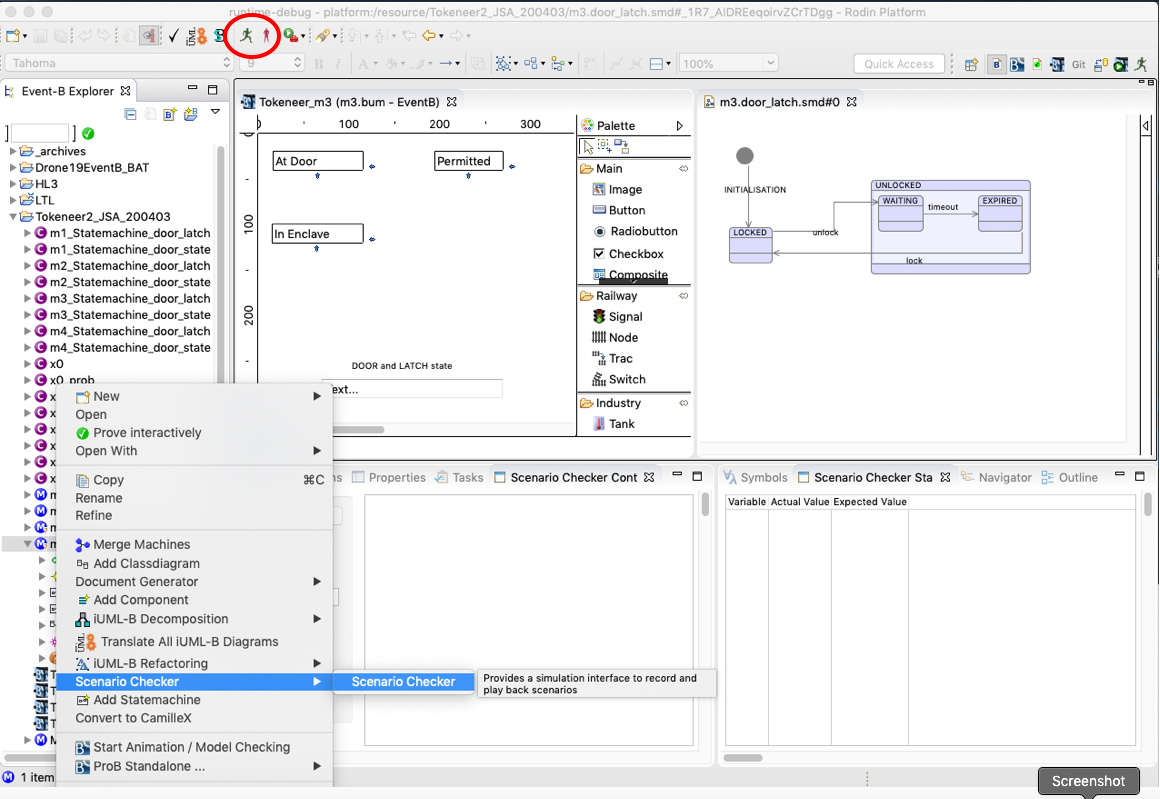
\includegraphics[width=512]{figures/starting}
  \else
  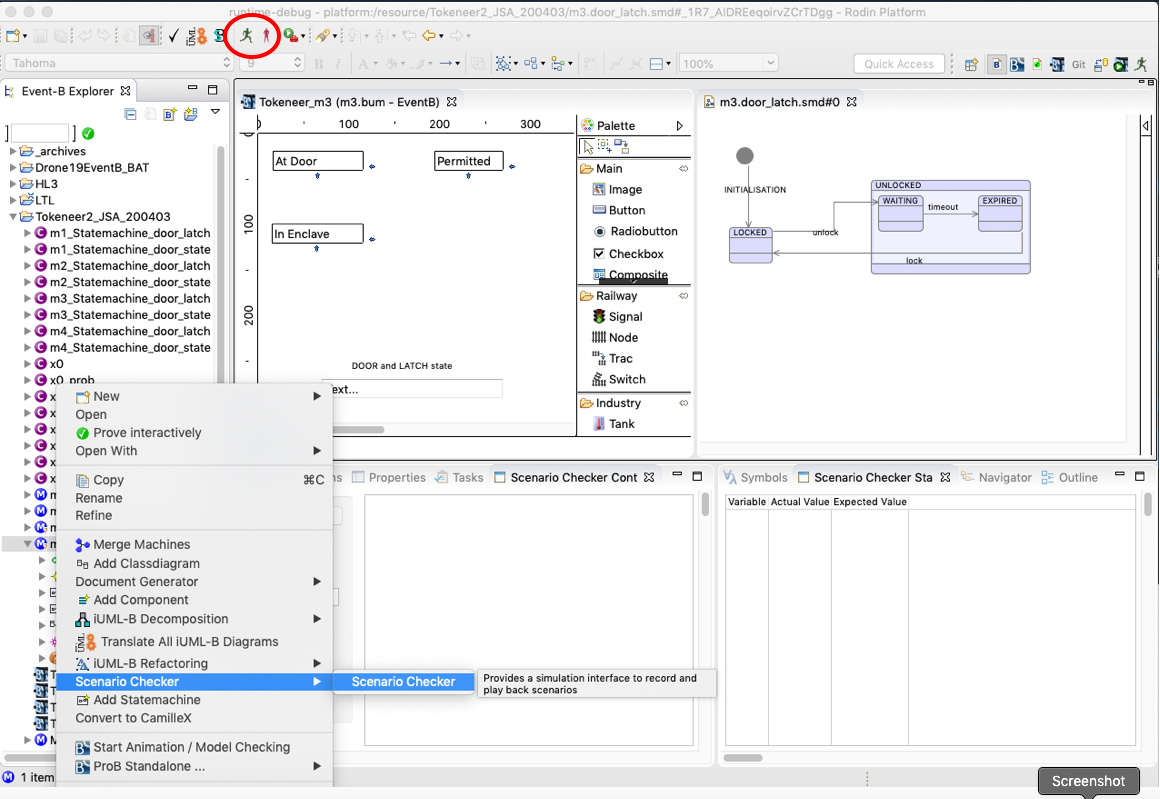
\includegraphics[width=0.9\textwidth]{figures/starting}
  \fi
  \caption{Starting the Scenario Checker}
  \label{fig:starting}
\end{figure}

\subsection{Setup}
\label{sec:setup}

The Scenario Checker always fires the ProB setup operation whenever it can (i.e. when it is started or re-started or replayed).
It is important for the sets and constants in the model, to be instantiated with suitable values to record a desired scenario.
The same values must also be instantiated in order for previously recorded scenarios to be replayed.
This can be done by adding an animation context that is seen by the machine to be animated.

\subsection{Persistence}
\label{sec:persistence}

Scenarios are persisted in the Oracle format.
This is an XML based format consisting of two types of elements which are expected to alternate.
Steps consist of the event signature that fired as part of the scenario
Snapshot records the state of changed variables and constants after the preceding steps.
The first step is always the ProB setup and this is followed by the first snapshot giving the values of sets and constants.
The second step is the initialisation followed by the snapshot giving the initial value of all variables.
After this the steps and snapshots depend on the scenario.
The oracle format is defined and generated from an EMF meta-model and hence is the default EMF XMI format for that meta-model.
Scenarios can be read and edited using an EMF editor such as Rose.


%%% Local Variables:
%%% mode: latex
%%% TeX-master: "user_manual"
%%% End:
